\documentclass[a4paper]{article}
\usepackage{amsfonts}
\usepackage{amsmath}
\usepackage{amssymb}
\usepackage{graphicx}     

\begin{document}
  
\noindent \large Auteur: CouldBeMathijs \\
\noindent \large Studierichting: Informatica\\
\noindent \large Oefeningenreeks 3H nr. 5.3\\

\medskip

\normalsize

$r = -\dfrac{3}{2}\cos \theta$\\

Periode van $2\pi$, we bekijken het interval $[0, 2\pi]$\\

Nulpunten r:\\

$0 = -\dfrac{3}{2}\cos \theta$\\

$\Rightarrow 0 = \cos \theta$\\

$\Rightarrow \theta_1 = \dfrac{\pi}{2}$ en $\theta_2 = \dfrac{3\pi}{2}$\\

Nulpunten afgeleide r:\\

$0 = \dfrac{3}{2} \sin \theta$\\

$\Rightarrow 0 = \sin \theta$\\

$\Rightarrow \theta_k = k \pi \quad \forall k \in \{0,1,2\}$\\

\begin{tabular}{c|ccccc}

	$\theta$   & $0$ & $\dfrac{\pi}{2}$  & $\pi$         & $\dfrac{3\pi}{2}$    & $2\pi$ \\ \hline

	$r$        & $-$ & $0$               & $+$           & $0$                  & $-$ \\

	$r'$       & $0$ & $+$               & $0$           & $-$                  & $0$ \\ \hline

    $r$        & $min1\left(-\dfrac{3}{2}\right)$ & $\nearrow$  & $Max\left(\dfrac{3}{2}\right)$ & $\searrow$  & $min\left(-\dfrac{3}{2}\right)$ \\
\end{tabular}\\

\begin{figure}[h]
    \centering
    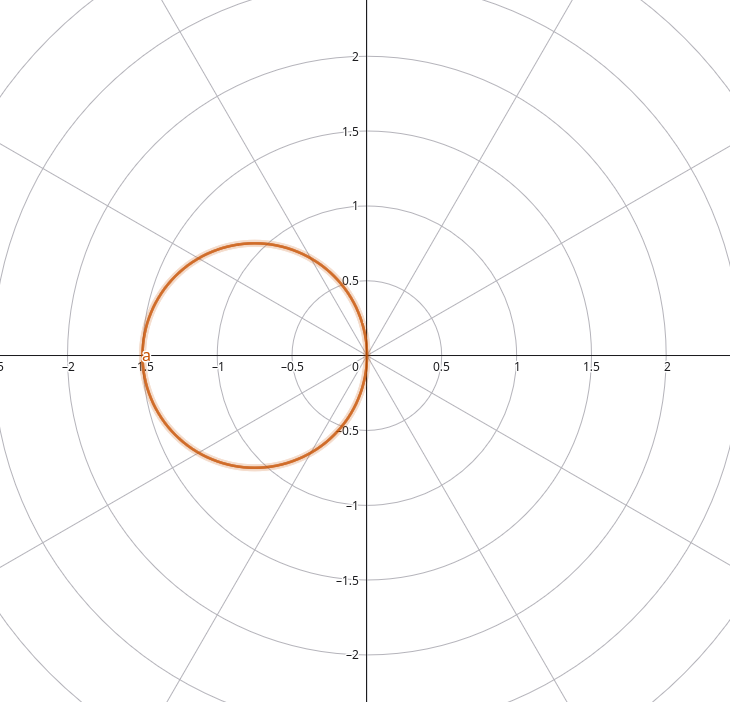
\includegraphics[width=5cm]{3H-5.3-could.be.mathijs.INF.png}
\end{figure}


\begin{thebibliography}{999}
%\bibitem{a} Referentie
\end{thebibliography}
\end{document} 
